% Partie 1.2 - Les différents protocoles et topologies %

\subsection{Les différents protocoles et topologies}

\subsubsection{Les différentes topologies}

Un réseau local (\textbf{LAN} pour \textit{Local Area Network}) est un réseau où les terminaux peuvent communiquer sans avoir besoin d'un accès à Internet. Mais il existe un autre type de réseau plus proche de nos contraintes, le réseau personnel (\textbf{PAN} pour \textit{Personal Area Network)}. Dans ce type de réseau, le but est de faire aboutir les échanges entre les divers éléments du réseau avec des puissances assez faible pour garantir une autonomie correcte, ce qui correspond bien à nos besoins avec les capteurs. Ils ont besoins d'être autonome le plus longtemps possible tout en évitant une interaction humaine physique directe.

Dans le monde des réseaux, nous utilisons le terme topologie pour définir l'arrangement des différents nœuds dans un réseau. Avec les réseaux PAN, on se limite assez souvent à deux topologies : le maillage partiel (\textit{mesh}) et le réseau en étoile (\textit{star}).

\begin{figure}[H]
\centering
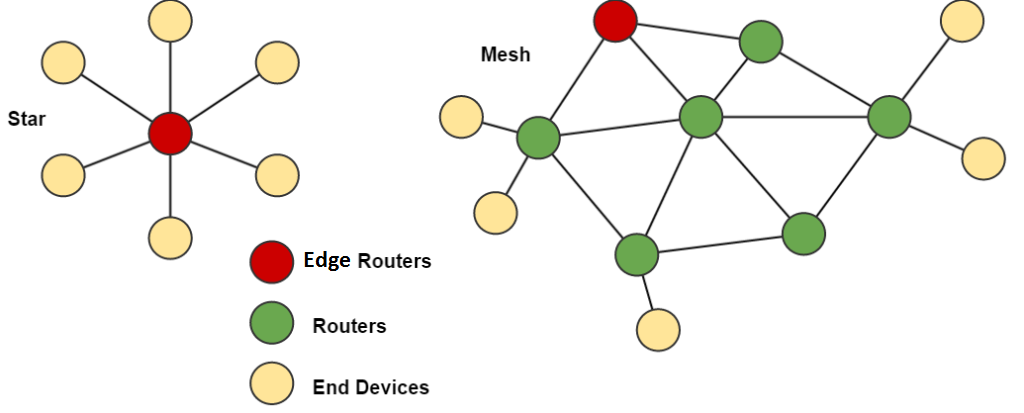
\includegraphics[width=15cm]{\rpDossier/images/topologies.png}
\caption{Comparaison des différentes topologies}
\label{topologies}
\end{figure}

La topologie en étoile (à droite sur la \cref{topologies}) est extrêmement repandue car c'est celle qui est utilisée dans le modèle maître/esclave. Le maître étant le point névralgique du réseau, toutes les communications sont obligées de passer par lui. Cela se révèle assez pratique dans le cas de la collecte de données car le maître est le point de convergence en plus d'être le point de sortie du réseau.

Cette topologie est en parfaite opposition avec le maillage partiel (à gauche sur la \cref{topologies}). En effet, dans cette dernière topologie, chaque nœud est potentiellement un routeur et chaque routeur un potentiel point de sortie. Ces derniers sont appelés des \textit{Edge Routers} ou \textit{Border Routers} et font le lien entre le PAN et d'autres réseaux. Les nœuds qui ne routent pas les paquets sont quant à eux appelés \textit{End Devices} ; c’est souvent le cas d’appareils peu puissants ne pouvant pas implémenter les algorithmes de routage.

Le fait est que, comme cette technologie est explorée par plusieurs constructeurs et organismes, plusieurs protocoles ont vu le jour, mais sans réel standard : chacun utilise celui qu'il veut. Cela pose pas mal de problème pour l'interopérabilité des éléments composants le réseau, ce qui est pourtant une des caractéristiques phare de l'IoT.

\subsubsection{les différents protocoles}

Dans cette partie, nous allons vous présenter divers protocoles orientés basse consommation. Ces protocoles sont développés par divers organismes, ce qui fait qu'aucun n'est un standard. Les constructeurs implémentent ceux qu’ils veulent. Cela peut poser certains problèmes d'interopérabilité et augmenter fortement le prix des appareils.

\begin{description}
	\item[Wi-Fi]
	Technologie sans fil permettant d'obtenir de gros débits, majoritairement utilisée pour donner un accès réseau à des équipements sans fil. Certaine variantes existent, comme \textit{Wi-Fi Direct}, qui permet le transfert de fichier à haute vitesse entre deux équipements. Le protocole est actuellement très énergivore, ce qui fait de cette technologie un mauvais candidat pour l'IoT, mais des groupes de travail cherchent à faire évoluer la norme (débit, bande-passante, consommation, vitesse d'association) en correspondance avec l'IoT pour gagner des parts de marché.

	\item[Bluetooth]
	Protocole sans fil opérant dans la bande 2,4 GHz. Il a été conçu pour l'échange de données sur de courtes distances mais ne tenait pas bien compte de la consommation. Généralement, un \textit{dongle} USB permettait l'ajout du bluetooth à son PC mais la technologie est devenue tellement commune qu'elle est maintenant complètement intégrée dans le matériel. Bluetooth utilise exclusivement une topologie en étoile, ce qui n'est pas très pratique pour l'établissement de grands réseaux (en termes de nombre de nœuds et de surface couverte).

	Le groupe travaillant sur Bluetooth changea la donne avec la quatrième version du protocole, qui introduit le \textit{Bluetooth Low Energy} (\textbf{BLE}, aussi connu sous le nom de \textit{Bluetooth Smart}). Cette version du protocole prend mieux en compte les besoins et contraintes de l'IoT, par exemple la consommation énergétique. La topologie en étoile est toujours obligatoire, mais un groupe d'étude a été lancé par \textit{Bluetooth \textbf{SIG}} (\textit{Special Interest Group}, les personnes en charge du développement de Bluetooth), nommé \textit{Smart Mesh}, qui a pour but de définir un standard pour pouvoir utiliser BLE avec une topologie maillée.

	\item[Zigbee]
	Ce protocole repose sur les couches basses définies par \textbf{802.15.4} (aussi utilisé par 6LoWPAN et défini dans la partie suivante). Il permet d’utiliser des topologies en étoiles et maillées, mais nécessite qu’un des équipements ait le rôle de « coordinateur ». Le coordinateur est généralement l'appareil avec le plus de puissance et il est la racine du réseau ; il peut avoir plusieurs rôles, comme faire la liaison entre réseaux ou servir d’aire de stockage pour les clés de sécurité. Il ne peut y avoir qu'un seul coordinateur par réseau et, dans le cas d'un réseau en étoile, il est forcément au centre.

	La technologie utilisant ce protocole est conçue comme une alternative plus simple et moins chère que celles des autres WPANs, comme Bluetooth ou Wi-Fi. La portée varie beaucoup en fonction de la bande de fréquence utilisé mais à titre d'exemple, la portée à 2,4 GHz en intérieur va de dix à vingt mètres. Les débits sont aussi relativement faibles : 20 kbit/s si l'on opère dans la bande 868 MHz et 250 kbit/s à 2,4 GHz. Les faibles débits permettent de maintenir une consommation extrêmement faible, ce qui permet aux équipements de tenir plusieurs années.	

	\item[Z-Wave]
	Protocole orienté domotique (automatisation dans les bâtiments) avec lequel chaque réseau peut comporter jusqu'à 232 noeuds ; la majorité de ces nœuds  sont des esclaves et les autres sont des contrôleurs. La topologie maillée implémente un système de saut (\textit{hop}), jusqu'à quatre, ce qui fait qu'avec une portée de base de 100 m plus les sauts, la couverture en terme de surface est très grande.

	Dans les dernières version de Z-Wave, un système d'\textit{explorer frame} (trame exploratoire) permet de réparer des routes quand un appareil est défectueux ou disparaît du réseau. Par contre, comme le protocole est routé statiquement, Z-Wave suppose que tous les appareils dans le réseau restent à leur place originelle. Les appareils mobiles, comme les télécommandes, sont donc impossibles à router.
\end{description}

Il existe beaucoup d'autres protocoles que nous ne développerons pas car leur usage reste assez limité.
